\hypertarget{Approach}{
}
In this section, the data and methods used for the experimental setup are outlined.

\section{PhoTex Database}\label{Photex}
The PhoTex database is created for physics-based computer vision. It provides excellent photometric data for texture classification, since all image data is  created under controlled conditions. The materials were recorded under a fixed view and different illumination angles. It also provides the materials under a rotated angle, but these images are discarded for the experiments conducted in this research. The most important features of the database for this research are:
\begin{itemize}
	\item Images are monochromatic.
	\item Resolution: 512 x 512
	\item Fixed and linear gain: images measured under different lighting conditions are comparable. 
\end{itemize}

\noindent The database mainly holds images of rough surfaces, and a few smooth surfaces. For all the image data, the azimuth and zenith angles of the light source are provided (these angles are also mentioned as slant and tilt), making it perfect for photometric stereo algorithms to recover the surface and albedo of the materials. The general setup for recording the materials can be seen in figure \ref{fig:PHOTEX_SETUP}. 

The images used in Targhi's experiment are chosen to have a high degree of diffuse reflection properties. All 20 classes are shown in figure X. In order to deal with possible illumination changes of novel data, it is desirable to preprocess the images such that they are intensity invariant by setting the images to zero-mean and unit-variance. 


\begin{figure}[H]
	\begin{center}
		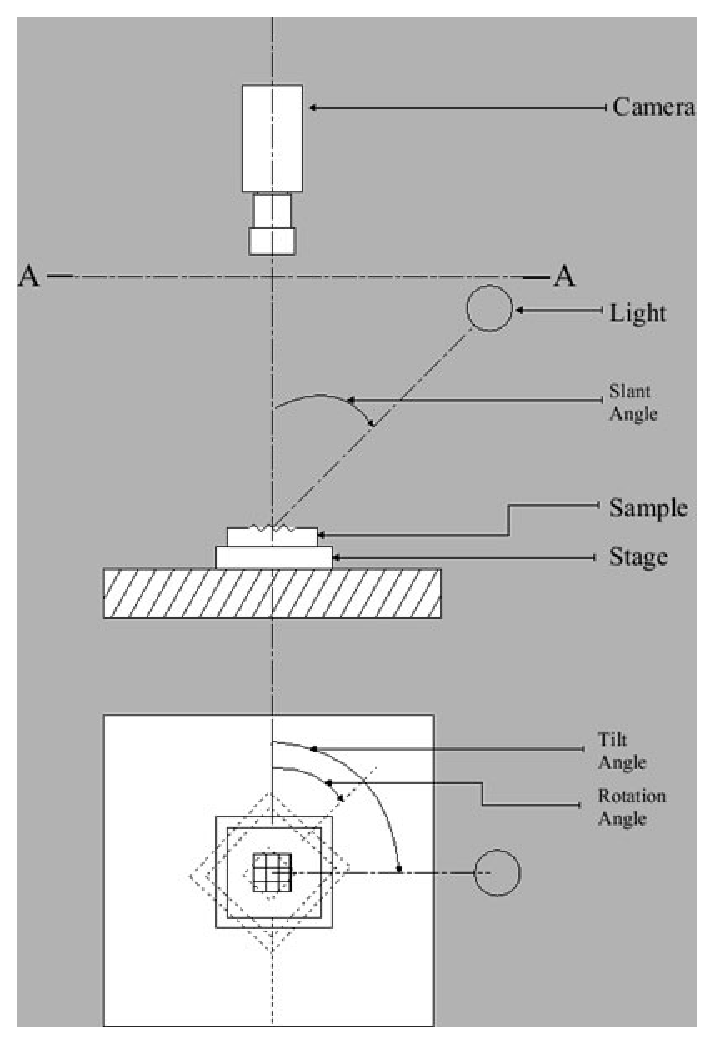
\epsfig{file=images/photex_setup.eps, width=0.5\linewidth}
	\end{center}
	\caption{Experimental setup of the recording of the PhoTex Database. Courtesy TextureLab @ Heriot-Watt University}
	\label{fig:PHOTEX_SETUP}
\end{figure}


http://www.macs.hw.ac.uk/texturelab/

\section{Photometric Stereo}\label{PhotometricStereo}

\begin{itemize}
	\item{core formula(s)}
	\item{Lambertian assumption}
\end{itemize}


\section{Classification}
\begin{itemize}
	\item{multivariate Gaussian Classifier, Mallow distance}
	\item{Texton Dictionary, Chi-distance}
\end{itemize}

